\documentclass[12pt, dutch, a4paper]{article}

\usepackage[hidelinks]{hyperref}
\usepackage[tmargin=0.8in, bmargin=1in]{geometry}
\usepackage{parskip}
\usepackage{amssymb}
\usepackage{amsmath}
\usepackage[shortlabels]{enumitem}
\usepackage[dutch]{babel}
\selectlanguage{dutch}
\usepackage{amsthm}
\usepackage{cleveref}
\usepackage{graphicx}
\usepackage{siunitx}

\theoremstyle{definition}

\newtheorem{theorem}{Stelling}
\newtheorem{lemma}{Lemma}[theorem]
\newtheorem{lemmalos}{Lemma}
\newtheorem{sublemma}{Lemma}[lemma]
\newtheorem{case}{Geval}
\newtheorem{claim}{Claim}

\newenvironment{shortclaim}
  {\refstepcounter{claim}\textbf{Claim~\theclaim.}}% \begin{shortthm}
{\enskip}
\newenvironment{shortthm}
  {\refstepcounter{theorem}\textbf{Stelling~\thetheorem.}}% \begin{shortthm}
{\enskip}

\usepackage[newfloat]{minted}
\usepackage[
  skip=0pt
  ]{caption}

\newenvironment{code}{\captionsetup{type=listing}}{}
\SetupFloatingEnvironment{listing}{placement=htp}
\SetupFloatingEnvironment{listing}{name=Code blok}

\title{Data V - inleveropdracht 1}
\author{Boris van Boxtel, Brechtje Poppen, \\  Floris Oostenbrug, Lotte Gritter}
\date{9 December 2022 - Week 49} 

\begin{document}

\maketitle  
\pagenumbering{arabic} 

\begin{enumerate}[(a.)]
\item \label{opdrA} Om de gemiddelde valtijd te berekenen gebruiken we python. Ook berekenen we de standaarddeviatie door middel van python. Dit geeft een waarde voor de gemiddelde valtijd ($\bar t$) van 72.9 in honderdste secondes en voor de standaarddeviatie ($\sigma_t$) van 7.037627805461519 in honderdste secondes. 

Dit doen we met de volgende code:
\newline
\begin{code}
  \caption{Code opdracht \ref{opdrA}}
  \inputminted[
    firstline=5,
    lastline=25,
    frame=lines, 
    breaklines,
    linenos,
    ]{python}{code/DataV_inlever1.py}
\end{code}

We gebruiken nu de tien procent regel om de standaarddeviatie correct af te ronden. Hiertoe ronden we de onzekerheid eerst af op twee decimalen, dus $\sigma_t$ = 7.04/100 s. Wanneer we dit nu op één decimaal afronden krijgen we 7.0/100 s. Volgens de tien procent regel mag je alleen op één decimaal afronden als hierdoor de afrondingsfout kleiner is dan tien procent van de onzekerheid in twee decimalen omdat er dan geen significant verlies van informatie is. Tien procent van de onzekerheid in twee decimalen is 0.704/100 s en de afrondingsfout is 0.04/100 s, wat veel kleiner is dan 0.704/100 s. De onzekerheid is dus 7.0/100 s. Dit betekent dat de gemiddelde valtijd afgerond moet worden op 73/100 s. 

De waarde van $\bar t$ is dus $(73 \pm 7.0)/100$ s.

\item \label{opdrB} 
We laten de meetresultaten hier in de vorm van een genormeerd histogram zien. Volgens de vuistregel van het aantal bins nemen we 6 bins, want $\text{round}(\sqrt{40}) = 6$.

\begin{figure}[h]
  \caption{Histogram van valtijden}
  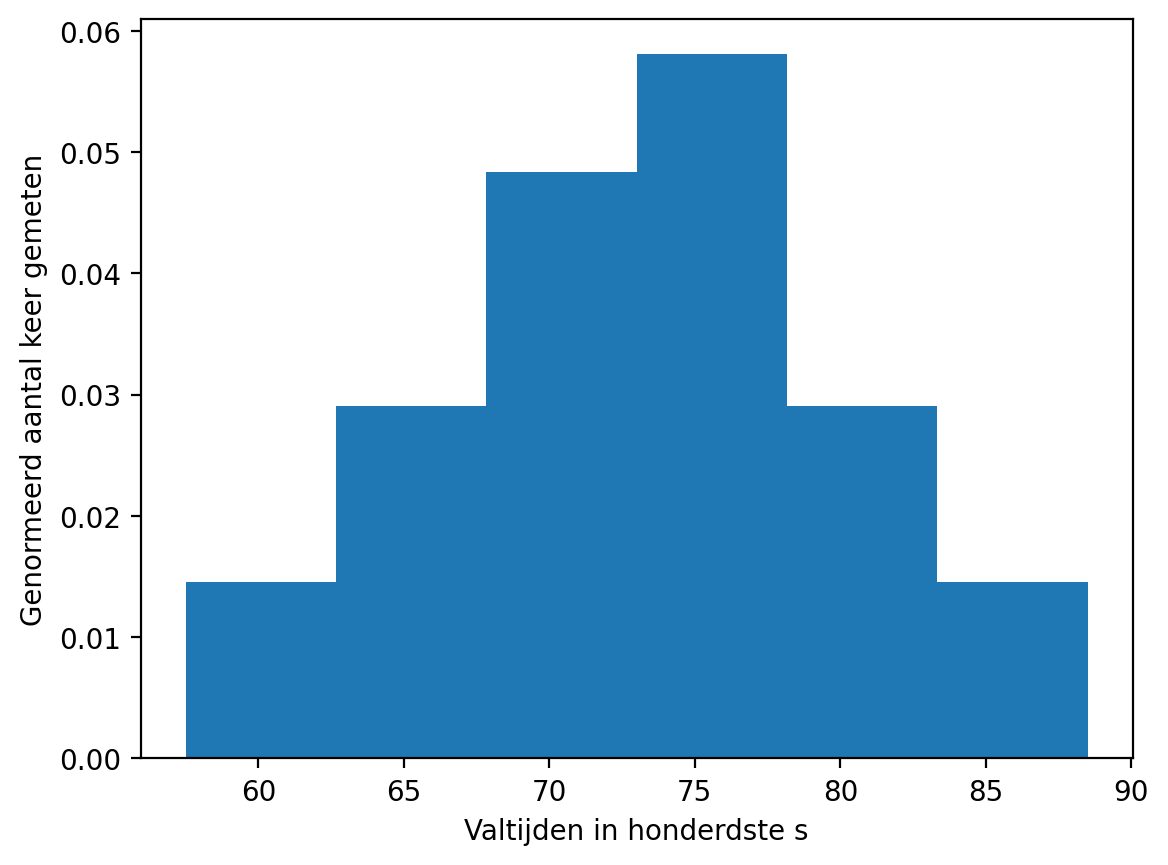
\includegraphics[scale=0.8]{images/normalized_histogram_valtijden.png}  
  \centering
\end{figure}

We berekenen nu  $\bar t_1$, ...,  $\bar t_{10}$ voor de 4 metingen in elk van de 10 kolommen door middel van python. 
Dit geeft de waardes:
$\bar t_1$ = 74.25/100 s,
$\bar t_2$ = 67.75/100 s,
$\bar t_3$ = 72.5/100 s,
$\bar t_4$ = 77.25/100 s,
$\bar t_5$ = 66.25/100 s,
$\bar t_6$ = 74.75/100 s,
$\bar t_7$ = 75.75/100 s,
$\bar t_8$ = 76.00/100 s,
$\bar t_9$ = 71.75/100 s en
$\bar t_{10}$ = 72.75/100 s.

Dit hebben we gevonden met de volgende code:
\newline
\begin{code}
  \caption{Code opdracht \ref{opdrB}}
  \inputminted[
    firstline=28,
    lastline=36,
    frame=lines, 
    breaklines,
    linenos,
    ]{python}{code/DataV_inlever1.py}
\end{code}
 
\item \label{opdrC}
We hebben in python het gemiddelde ($\bar t_{deel}$) en de bijbehorende standaarddeviatie ($\sigma_{deel}$) berekend. Dit gaf de waardes $\bar t_{deel}$ = 72.9 in honderste secondes en $\sigma_{deel}$ = 3.561366778827103 in honderste secondes. 

Dit hebben we gevonden met de volgende code:
\newline
\begin{code}
  \caption{Code opdracht \ref{opdrC}}
  \inputminted[
    firstline=49,
    lastline=52,
    frame=lines, 
    breaklines,
    linenos,
    ]{python}{code/DataV_inlever1.py}
\end{code}

We gebruiken nu de van procent regel om de standaarddeviatie goed af te ronden. We ronden de standaarddeviatie eerst af op 3.56/100 s. Wanneer we dit op 3.6/100 s afronden is de afrondfout gelijk aan 0.04/100 s. Tien procent van 3.56/100 s is gelijk aan 0.356/100 s. De afrondingsfout van 0.04/100 s is veel kleiner dan 0.356/100 s dus we ronden de standaarddeviatie af op 3.56/100 s. Dit betekent dat $\bar t_{deel}$ afgerond wordt naar 73/100 s. 

Het is wel te verwachten dat het gemiddelde van de valtijden berekend in \ref{opdrA} gelijk is aan het zojuist berekende $\bar t_{deel}$. Dit is ook het geval. Dit is te verwachten omdat we bij opdracht \ref{opdrA} de som van $t_1, ..., t_{40}$ hebben gedeeld door 40. We hebben dus de berekening $\frac{1}{40}\Sigma_{n=1}^{40} t_n = \bar t$ gedaan om $\bar t$ te krijgen. 

In opdracht \ref{opdrB} hebben we toen de berekeningen $\frac{1}{4}\Sigma_{n=1}^{4} t_n = \bar t_1$, $\frac{1}{4}\Sigma_{n=5}^{8} t_n = \bar t_2$, .. , $\frac{1}{4}\Sigma_{n=37}^{40} t_n = \bar t_{10}$ gedaan om $\bar t_1, ..., \bar t_{10}$ te krijgen. 

Toen hebben we in opdracht \ref{opdrC} de berekening $\frac{1}{10}\Sigma_{n=1}^{10} \bar t_n = \bar t_{deel}$ gedaan om $\bar t_{deel}$ te krijgen. 

De berekening die in opdracht \ref{opdrC} is gedaan is te schrijven als $\frac{1}{10} \cdot (\frac{1}{4}\Sigma_{n=1}^{4} t_n + \frac{1}{4}\Sigma_{n=5}^{8} t_n + ... + \frac{1}{4}\Sigma_{n=37}^{40} t_n) = \frac{1}{40} \cdot (\Sigma_{n=1}^{4} t_n + \Sigma_{n=5}^{8} t_n + ... + \Sigma_{n=37}^{40} t_n) =  \frac{1}{40} \Sigma_{n=1}^{40} t_i$. De berekening die we bij \ref{opdrC} hebben gedaan is dus gelijk aan de berekening die we bij \ref{opdrA} deden en dus is het te verwachten dat de uitkomst gelijk is.

Het is echter niet te verwachten dat de uitkomst voor de standaarddeviatie bij \ref{opdrA} en \ref{opdrC} gelijk zou zijn. Dit is ook niet het geval. 

Wanneer namelijk het gemiddelde van vier valtijden genomen wordt ligt de uitkomst dichter bij de werkelijke valtijd dan elk van de vier losse metingen. De waardes waarvan het gemiddelde werd genomen in \ref{opdrC} lagen dus allemaal al dichter bij de werkelijke valtijd dan de losse metingen bij \ref{opdrA}. Hoe dichter de waardes waarover de standaarddeviatie wordt berekend bij het werkelijke gemiddelde liggen, hoe kleiner de standaarddeviatie. De standaarddeviaitie bij \ref{opdrC} was inderdaad kleiner dan bij \ref{opdrA}.

\newpage
\item \label{opdrD} 
Twee metingen $x_1, x_2$ van de valtijd zijn consistent met elkaar als het volgende geldt: $\lvert x_1 - x_2 \rvert \leq 2\sigma_{t}$. Twee metingen zijn strijdig als geldt $\lvert x_1 - x_2 \rvert > 2\sigma_{t}$. Twee correcte metingen kunnen strijdig zijn, er bestaat namelijk een kleine kans dat twee metingen meer dan $2\sigma_{t}$ uit elkaar liggen. De standaarddeviatie $\sigma_{t}$ is bij \ref{opdrA} berekend en bedraagt 7.0/100 s. Er geldt voor $t_5$ en $t_8$ dat $\lvert t_5 - t_8 \rvert = \lvert 70/100 \unit{\second} - 82/100 \unit{\second} \rvert = 12/100 \unit{\second} < 14/100 \unit{\second} = 2\sigma_{t}$. De twee metingen zijn dus niet strijdig. 

% Wanneer twee metingen consistent zijn met elkaar kunnen ze door rekening te houden met de onzekerheid dezelfde waarde hebben. Wanneer twee metingen strijdig zijn kunnen ze niet dezelfde waarde hebben wanneer er rekening gehouden wordt met de onzekerheid. Er geldt: $t_5 = (70 \pm 7.0)/100$ s en $t_8 = (68 \pm 7.0)/100$ s. Aangezien de waarde van $t_5$ tussen 63.0/100 s en 77.0/100 s ligt en die van $t_8$ tussen 61.0/100 s en 75.0/100 s kunnen ze dezelfde waarde hebben. De resultaten $t_5$ en $t_8$ zijn dus consistent. (niet af)

% Wanneer twee metingen consistent zijn met elkaar kunnen ze door de onzekerheid dezelfde waarde hebben. Wanneer twee metingen strijdig zijn kunnen ze niet dezelfde waarde hebben, zelfs niet wanneer er rekening gehouden wordt met de onzekerheid. Aangezien de waarde van $t_5$ tussen 63.0/100 s en 77.0/100 s ligt en die van $t_8$ tussen 61.0/100 s en 75.0/100 s kunnen ze dezelfde waarde hebben. De resultaten $t_5$ en $t_8$ zijn dus consistent. (niet af)

\end{enumerate}

\end{document}